\documentclass[aspectratio=1609]{beamer}

%Style


%Packages
\usepackage[utf8]{inputenc}
\usepackage{color}
\usepackage{graphicx}
\usepackage{booktabs}
\usepackage{lmodern}
\usepackage{amsfonts,amsmath,amssymb,amsthm}
\usepackage{varwidth}
\usepackage{mathtools}
\usepackage{xcolor}
\usepackage{framed}
\definecolor{shadecolor}{RGB}{180,180,180}
\usepackage{pgfplots}
\usetikzlibrary{arrows.meta}
\usepgfplotslibrary{groupplots}
\pgfplotsset{compat=newest}
\usetheme{HM}


%Title and Footer----------------------------------
\title[Enhanced PDR for Firefighting]{Enhanced Pedestrian Dead Reckoning Sensor Fusion for Firefighting}
\author{Tobias Augustin, Daniel Ossmann}
\institute[]{University of Applied Science Munich, HM}
\date{\today}
%--------------------------------------------------

\definecolor{HMRed}{RGB}{252 085 085}
\definecolor{HMRed2}{RGB}{254 184 184}
\definecolor{MYgray}{RGB}{140 136 136}
\definecolor{FK03}{RGB}{000,141,208}
\definecolor{lightgrey}{RGB}{207 200 200}
\definecolor{lightergrey}{RGB}{209, 207, 207}
\definecolor{green}{RGB}{013 189 016}
\definecolor{orange}{RGB}{235, 152, 052}
\definecolor{lila}{RGB}{162, 052, 235}

\definecolor{color2}{RGB}{65, 64, 112}

\definecolor{black}{RGB}{000 000 000}

\usetikzlibrary{positioning,plotmarks, matrix, arrows, calc, shapes}
\tikzstyle{blockdiag}	= [node distance=0mm, >=stealth', semithick]

%Hier beginnt die Präsentation
\begin{document}	
	% Title page frame
	{
	{\setbeamertemplate{footline}{}
	
		\begin{frame}
			\titlepage
		\end{frame}}
	\usebackgroundtemplate{ }
	
	\begin{frame}{Introduction}
		
	\end{frame}}
	
	\begin{frame}{Requirements for Firefighting}
		\begin{itemize}
			\item Does not require prior setup of electronics
			\item Should be able to work in smoke [Schlecht!]
			\item Lightweight and easy to carry
			\item 
		\end{itemize}
	\end{frame}
	
	\begin{frame}{Existing Solutions}
		Inhalt...
	\end{frame}
	
	\begin{frame}{Step-Detection}
		\begin{itemize}
			\item Zero-crossing detection 
			\item Step-length estimation with $d = \sqrt[4]{a_{\max}-a_{\min}}  \, c$
			\item Step-length is added in the direction the individual is looking
		\end{itemize}
		\vspace{0.5cm}
		\begin{figure}
			\centering
			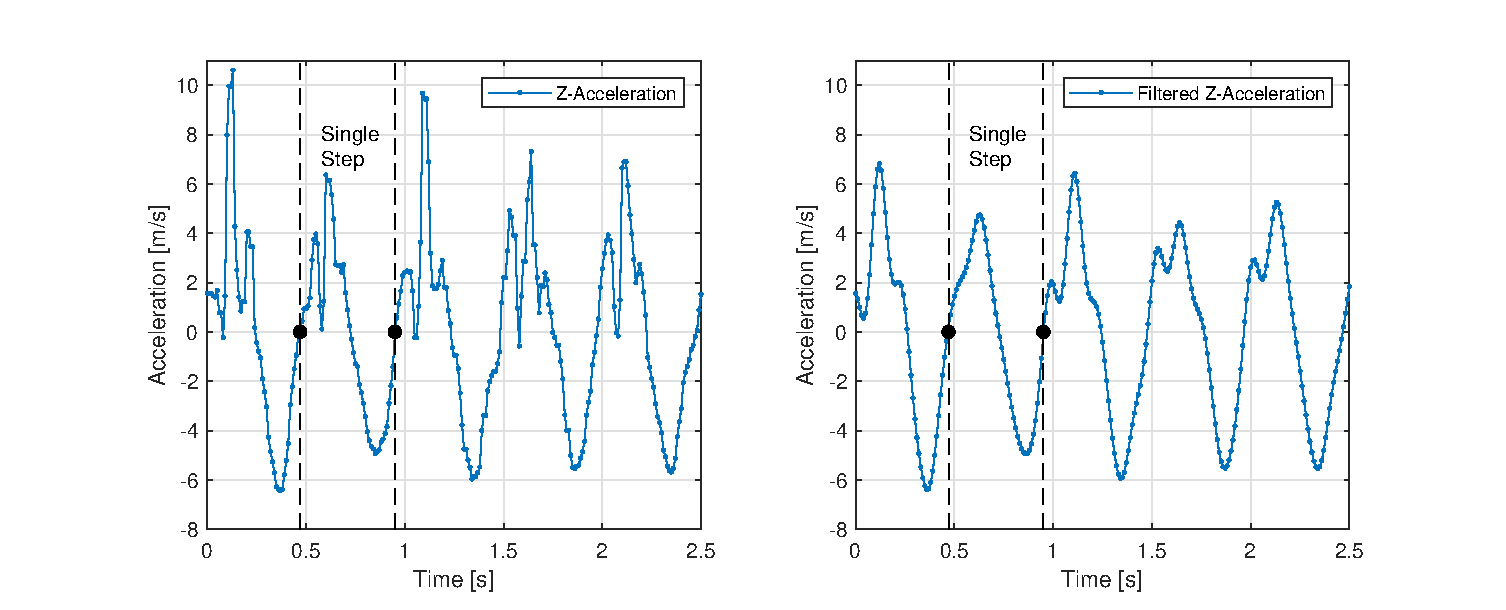
\includegraphics[width=0.9\linewidth]{../Conference_Paper/WalkAcceleration}
			\caption{}
			\label{fig:walkacceleration}
		\end{figure}
			

		
	\end{frame}
	
	\begin{frame}{Tracking Camera}
		\begin{itemize}
			\item Stereo-camera ...
			\item Works by tracking pixels and calculating the distance to them
			\item Intel RealSense T265 was used
		\end{itemize}
		\begin{figure}
			\centering
			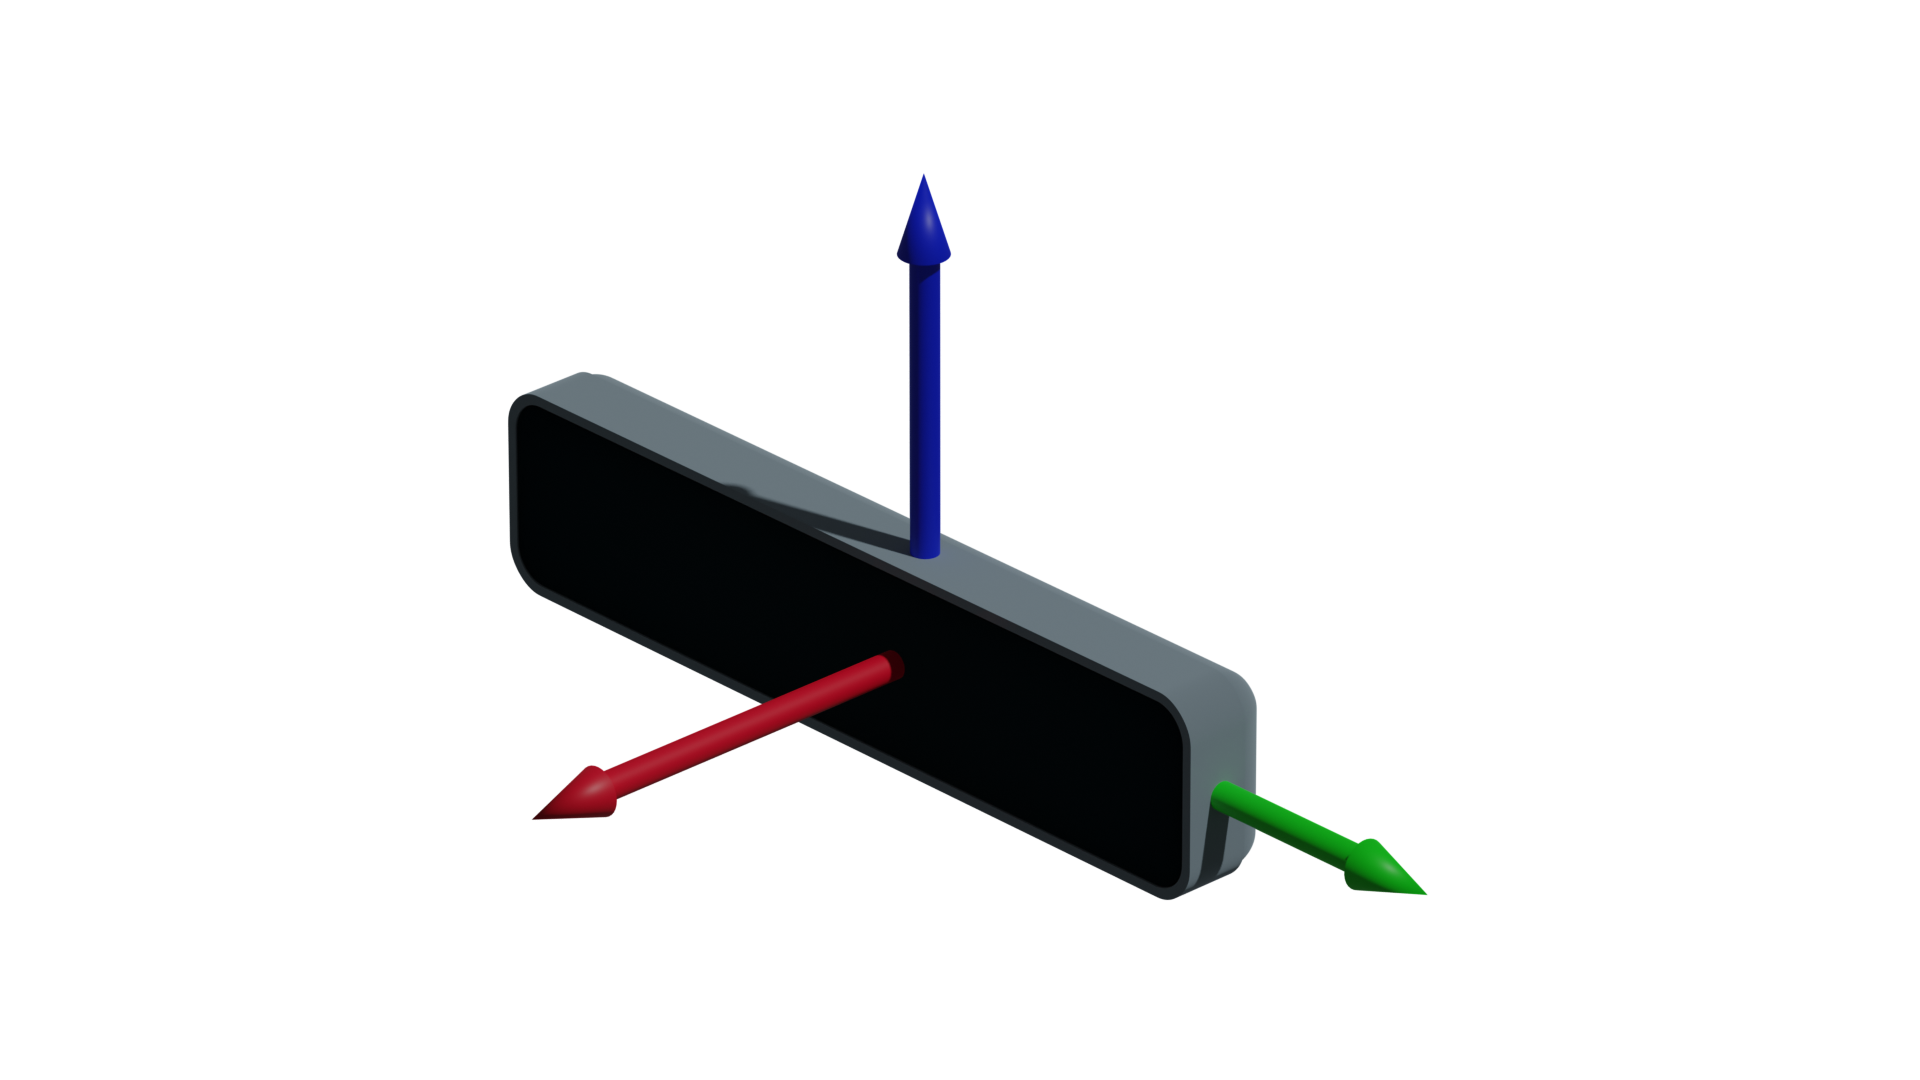
\includegraphics[width=0.7\textwidth]{../Conference_Paper/realsense.png}
		\end{figure}
	\end{frame}
	
	\begin{frame}{Sensor-Data Fusion}
		Inhalt...
	\end{frame}
	
	\begin{frame}{Design Evaluation}
		\begin{itemize}
			\item Only lab-tests as a proof of concept and to tune the system
			\item Walked or moved in a crouching movement on a set trajectory
			\item Analysis of the deviation on defined checkpoints
			\item Sensor assembly mounted on the backplate of a breathing apparatus
		\end{itemize}
		
	\end{frame}
	
	\begin{frame}{Results}
		\begin{columns}
			\begin{column}{0.45\textwidth}
				\begin{itemize}
					\item Text
				\end{itemize}
			\end{column}
			\begin{column}{0.54\textwidth}
				\begin{figure}
					\centering
					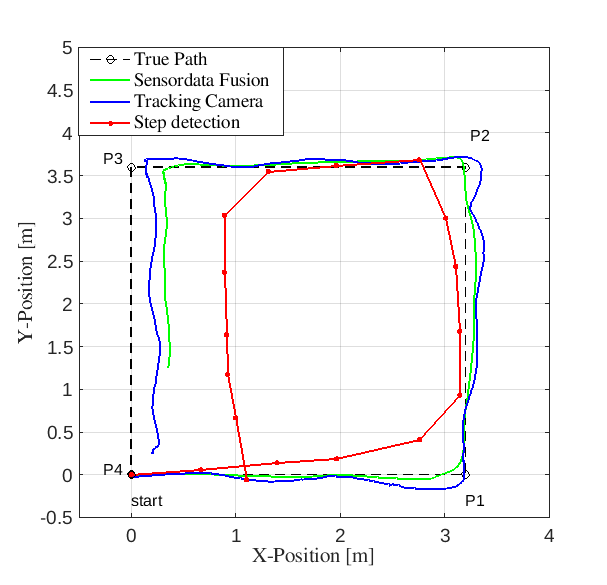
\includegraphics[width=0.9\linewidth]{../Conference_Paper/Path}
					\caption{}
					\label{fig:path}
				\end{figure}
			\end{column}
					
			
		\end{columns}
	\end{frame}
	
	\begin{frame}{What next?}
		\begin{itemize}
			\item Further tests in a firefighting environment are necessary
			\item[$\rightarrow$] Sensor assembly needs to be adapted for this task
		\end{itemize}
		
	\end{frame}

	
\end{document}